%
% FH Technikum Wien
% !TEX encoding = UTF-8 Unicode
%
% Erstellung von Master- und Bachelorarbeiten an der FH Technikum Wien mit Hilfe von LaTeX und der Klasse TWBOOK
%
% Um ein eigenes Dokument zu erstellen, müssen Sie folgendes ergänzen:
% 1) Mit \documentclass[..] einstellen: Master- oder Bachelorarbeit, Studiengang und Sprache
% 2) Mit \newcommand{\FHTWCitationType}.. Zitierstandard festlegen (wird in der Regel vom Studiengang vorgegeben - bitte erfragen)
% 3) Deckblatt, Kurzfassung, etc. ausfüllen
% 4) und die Arbeit schreiben (die verwendeten Literaturquellen in Literatur.bib eintragen)
%
% Getestet mit TeXstudio mit Zeichenkodierung ISO-8859-1 (=ansinew/latin1) und MikTex unter Windows
% Zu beachten ist, dass die Kodierung der Datei mit der Kodierung des paketes inputenc zusammen passt!
% Die Kodierung der Datei twbook.cls MUSS ANSI betragen!
% Bei der Verwendung von UTF8 muss dnicht nur die Kodierung des Dokuments auf UTF8 gestellt sein, sondern auch die des BibTex-Files!
%
% Bugreports und Feedback bitte per E-Mail an latex@technikum-wien.at
%
% Versionen
% *) V0.7: 9.1.2015, RO: Modeline angepasst und verschoben
% *) V0.6: 10.10.2014, RO: Weitere Anpassung an die UK
% *) V0.5: 8.8.2014, WK: Literaturquellen überarbeitet und angepasst
% *) V0.4: 4.8.2014, WK: Initalversion in SVN eingespielt
%
\documentclass[MSE,Master,english]{twbook}%\documentclass[Bachelor,BMR,ngerman]{twbook}
\usepackage[utf8]{inputenc}
\usepackage[T1]{fontenc}
\usepackage{float}

\newboolean{showImages} % Deklaration einer boolschen Variable
\setboolean{showImages}{true} % Zuweisung eines Wertes.

\newboolean{showListings} % Deklaration einer boolschen Variable
\setboolean{showListings}{true} % Zuweisung eines Wertes.

\newboolean{showTables} % Deklaration einer boolschen Variable
\setboolean{showTables}{true} % Zuweisung eines Wertes.

\newboolean{showUnusedContent} % Deklaration einer boolschen Variable
\setboolean{showUnusedContent}{false} % Zuweisung eines Wertes.


%
% Hier biblatex & Biber konfigurieren; Vergessen Sie nicht, dass Sie biber verwenden müssen um eine Bibliothek zu erzeugen
%
\usepackage[backend=biber, style=numeric]{biblatex}
\addbibresource{Literatur.bib}

%
% Bei Bedarf bitte hier die Syntax-Highlightings anpassen
%
\usepackage{minted}
\makeatletter
% Setzen der Bezeichnungen für das Quellcodeverzeichnis/Abkürzungsverzeichnis in Abhängigkeit von der eingestellten Sprache
\providecommand\listacroname{}
\@ifclasswith{twbook}{english}
{%
    \renewcommand\listoflistingscaption{List of source codes}
    \renewcommand\listacroname{List of Abbreviations}
}{%
    \renewcommand\listoflistingscaption{Quellcodeverzeichnis}
    \renewcommand\listacroname{Abkürzungsverzeichnis}
}
\makeatother

% Die nachfolgenden Pakete stellen sonst nicht benötigte Features zur Verfügung
\usepackage{blindtext}

%
% Einträge für Deckblatt, Kurzfassung, etc.
%
\title{Can GraphQL bring a performance improvement in micro-frontend architectures?}
\author{Florian Mold, BSc}
\studentnumber{11776836}
%\author{Titel Vorname Name, Titel\and{}Titel Vorname Name, Titel}
%\studentnumber{XXXXXXXXXXXXXXX\and{}XXXXXXXXXXXXXXX}
\supervisor{David Leitner, MSc}
%\supervisor[Begutachter]{Titel Vorname Name, Titel}
%\supervisor[Begutachterin]{Titel Vorname Name, Titel}
%\secondsupervisor{Titel Vorname Name, Titel}
%\secondsupervisor[Begutachter]{Titel Vorname Name, Titel}
%\secondsupervisor[Begutachterinnen]{Titel Vorname Name, Titel}
\place{Wien}
\kurzfassung{In diesem Projektbericht wird untersucht, ob eine Mikro-Frontend-Architektur von einer gemeinsamen Caching-Schicht profitieren kann. Außerdem wird untersucht, ob das Senden von einem Teil einer GraphQL Query an das GraphQL-Backend, welche Felder entfernt, die sich bereits im Cache befinden, einen Leistungsvorteil bietet. Der Prototyp wurde mit drei verschiedenen Ansätzen evaluiert und anhand der Anfrage- und Antwortgröße verglichen. Es wird diskutiert, ob die Vorteile der zusätzlichen Komplexität durch die Verbesserungen durch Caching die Nachteile überwiegen.}
\schlagworte{GraphQL, Micro-frontend, Caching, Backend-For-Frontend}
\outline{This project report evaluates whether a micro-frontend architecture can benefit from a shared caching layer. Furthermore, we evaluate whether sending partial queries to the GraphQL backend that remove fields that are already in the cache provides a performance benefit. The prototype was evaluated using three different approaches and compared based on query and response size. The debate is whether the benefits of the added complexity from the improvements through caching outweigh the disadvantages.}

\keywords{GraphQL, Micro-frontend, Caching, Backend-For-Frontend}
%\acknowledgements{\blindtext}

\begin{document}

\maketitle

\chapter{Introduction}\label{chapter:introduction}
 
The company AGnet has an outdated monolithic system to manage its customers, sales and so on. The technology stack is outdated which is why a migration to a newer technology is necessary. The new architecture should consist of micro-frontends and microservices. Some microservices are already in development, the micro-frontends should be prototyped in the course of this work. Micro-frontends have different problems than traditional frontend-applications. The prototype that is developed should tackle the problems that a distributed architecture brings to the table.
 
This project report is structured in a theoretical part. It is followed by a practical part. In the final chapters the results of the work are presented and discussed. This chapter describes the motivation the hypothesis and state-of-the-art solutions for the project report. Chapter \ref{chapter:applied-methods} covers the methods applied to optimize the number of requests and reduce the network-traffic. The results can be found in Chapter \ref{chapter:results} and the discussion resolving around the result is in Chapter \ref{chapter:discussion}. The final Chapter \ref{chapter:conclusion} concludes the report.

\section{State of the art}

This chapter provides information about state-of-the-art software architecture and integration styles relevant for this project. A short section is dedicated to every relevant technology of this report.

\subsection{Micro Frontends}

Micro-frontends should bring the same advantages of microservices from the backend to the frontend. Instead of creating a large frontend monolith, a micro-frontend architecture contains many small applications. The advantage is that every micro-frontend can be developed and deployed by a separate team. \cite{book:2020:geers:micro-frontends-in-action} The difference between frontend-monoliths and micro-frontends can be seen in figure \ref{figure:state-of-the-art:ui-monotlith-micro-frontend}.

\ifshowImages
\begin{figure}[H]
\centering
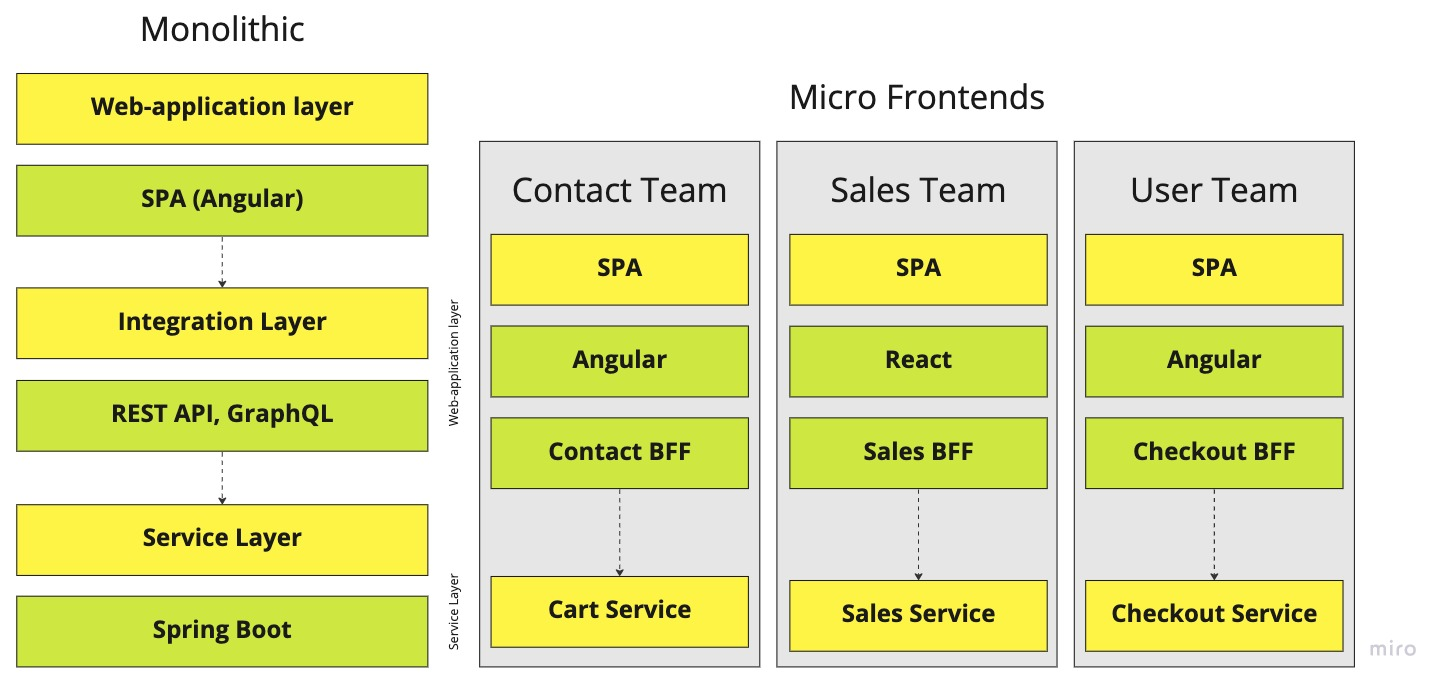
\includegraphics[width=0.8\linewidth]{images/ui-monotlith-micro-frontends.jpg}
\caption{A comparison between frontend-monoliths and micro-frontends.}\label{figure:state-of-the-art:ui-monotlith-micro-frontend}
\end{figure}
\fi


Benefits gained from working with microservices on the backend are lost, when working with a monolithical frontend. With a monolithic frontend, the ability to deploy independently is lost. The entire frontend has to be deployed at once. Another problem is, that distinct operations are not really possible. If one part of the frontend is broken, there is a good chance that the entire frontend is broken. Another problem is the parallel development. The speed of development cannot be increased because it is very difficult to have multiple teams working on one frontend application. \cite{misc:2019:leitner:micro-frontends}

The term micro-frontend can be misleading, as can the term microservice. It has no meaning in terms of the size of the application. It can be a simple widget that only displays data, or a full-blown one-page application. Ideally, a micro frontend covers an area of the entire frontend application.

\ifshowUnusedContent
% TODO(FM): Integration strategy not really important for short explaination
% Micro-frontends offer various strategies for integration. Integration means how the frontends are composed on the frontend. The web allows multiple strategies to incorporate the micro-frontends. 

% [1] M. Bischof and D. Leitner, “Analysis of the Suitability of a Microservice and a Micro-Frontend Architecture for an Existing Monolithic System,” p. 88.

% \begin{itemize}
%     \item Server Side Integration 
%     \item Client Side Integration
%     \item Build time Integration
% \end{itemize}

\fi

\subsection{Generic APIs vs Consumer Driven APIs}

The big decision in micro-frontend API development is to use either generic or consumer-oriented APIs. The difference is that generic APIs place great emphasis on reusability, while consumer-oriented APIs tailor the APIs to the customer.

\subsubsection{Generic APIs}

Generic APIs refer to APIs that are very general and can be used by different clients. However, this type of API has two major drawbacks. Over-fetching describes the problem of getting more data than is needed. Over-requesting describes the problem of needing multiple requests to get the data for a use case. Both problems are discussed in more detail in the next paragraphs. \cite{misc:2019:leitner:backend-for-frontends}

\paragraph{Over-Fetching}

For example, a contact service provides a contact-model that includes customer-number, first-name, second-name, uid-number and the address of the user, as seen in listing \ref{code:state-art:over-fetching}. However, one requirement of the application is to display only a contact's first and last name inside the header. Only two fields of the model are used, and the rest are unnecessarily queried. \cite{misc:2019:leitner:backend-for-frontends}

\ifshowListings
\begin{listing}[H]
\begin{minted}{typescript}
interface ContactModel {
  id: string;
  customerNumber: string;
  firstName: string;
  secondName: string;
  uidNumber: string;

  Address: {
    id: string;
    postalCode: string;
    location: string;
    Country: string;
  }
}
\end{minted}
\caption{Contact-Model that contains too much fields for the requirement.}\label{code:state-art:over-fetching}
\end{listing}
\fi

\paragraph{Over-Requesting}

Attempting to solve the problem of over-fetching by reducing the amount of data set that is returned leads directly to this problem. Listing \ref{code:state-art:over-requesting} shows the problem of over-requesting. If another requirement inside the application should display the address alongside the contact, two requests have to be performed every time. Afterwards, the two data sets have to be merged, which leads to high complexity on the client side. \cite{misc:2019:leitner:backend-for-frontends}

\ifshowListings
\begin{listing}[H]
\begin{minted}{typescript}
interface ContactModel {
  id: string;
  customerNumber: string;
  firstName: string;
  secondName: string;
  uidNumber: string;

  address_id: string;
}
\end{minted}
\caption{Contact-Model model that links the address-model with an id.}\label{code:state-art:over-requesting}
\end{listing}
\fi

\subsubsection{Consumer Driven APIs}

Consumer-driven APIs are the opposite of generic APIs. They follow the idea of providing the client with exactly the data it needs. Following the example above, the contact service would have an endpoint that returns only the first and last name as required for the request. These endpoints make communication with a client very simple and there is not the problem of over-fetching and over-requesting. However, creating an endpoint for each request creates an unmanageable set of endpoints. \cite{misc:2019:leitner:backend-for-frontends}

\subsubsection{Backend for Frontend}

\ifshowUnusedContent
% TODO(FM): Too specific for the project report.
% Every microservice provides its functionality to consumers with APIs. But it is not advisable that clients directly communicate with microservice APIs. Microservice offer fine-grained interfaces which were made especially for the communication between microservices. Therefore, the client usually has to make multiple requests to fetch the data needed for a view. ([7] S. Newman, Building microservices: designing fine-grained systems, First Edition. Beijing Sebastopol, CA: O’Reilly Media, 2015, (ISBN 978-1-4919-5035-7).

% This leads to many requests, which is also known as over-requesting.

% Another problem could be that a cluster of microservices use another form of communication. For example an asynchronous message-bus or another protocol like GRPC. There is the next problem. Clients usually communicate using synchronous communication, where microservices could use asynchronous communication. Without an adapter in between, the communication will not work properly. Even if the communication is possible, the client needs to know many details (IP-address) about the cluster of microservices. And the client might have to connect to multiple microservice to fetch the data needed to display one view. Therefore the client has to join the data in-memory. Changing the API of a microservice would have a ripple effect on the requests on the frontends, because they would have to be changed in many places.

% [1] C. Richardson, Microservices patterns: with examples in Java. Shelter Island, New York: Manning Publications, 2019, (ISBN 978-1-61729-454-9).

% To solve this problem the clients communicate with an API gateway or a more client centric backend-for-frontend service. Internally these services communicate with the microservice-cluster. An API gateway is a service that represents an abstraction of the microservice APIs and is an entry point to the microservice-cluster. The main task of a gateway is to forward tasks to the correct microservice. The even might implement functionalities like authorization and authentication or transform the protocol. Like transforming HTTP to GRPC. With API gateways it is also easier to split a microservice into two for example, without a ripple effect to change all clients as well.

% But the problem with API gateways is the ownership. Multiple teams will add their functionality to the gateway and might come into conflict. The APIs are often not suited for the needs of clients and it has to be avoided that client logic is developed into the API gateway.


% ([14] P. Siriwardena and N. Dias, Microservices security in action. Manning Publications, 2020, (ISBN 978-1-61729-595-9).)

% ([12] M. Geers, Micro Frontends in Action. Manning Publications, 2020)
\fi

To solve these problems, the backend-for-frontend pattern is often used. This pattern provides each client with its own API, which specialized for the needs of the client. \cite{book:2018:richardson:microservices-patterns}

\ifshowImages
\begin{figure}[H]
\centering
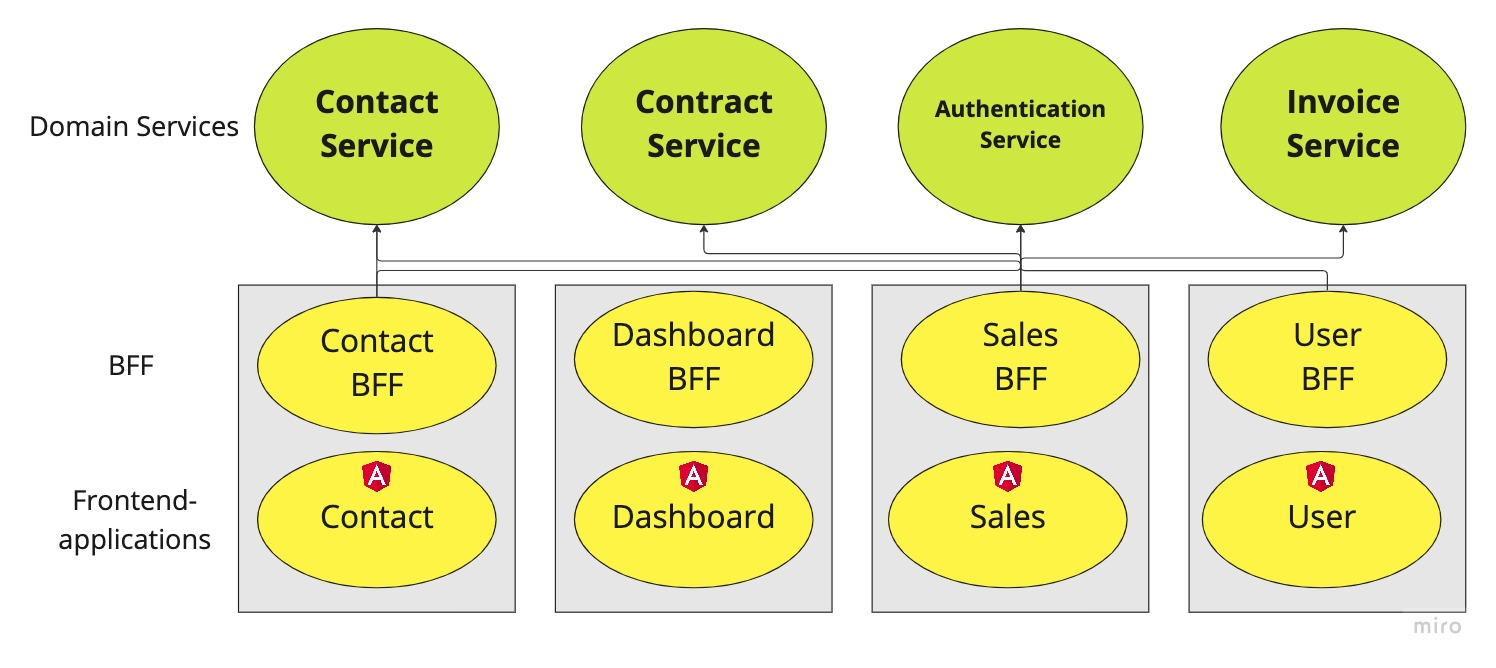
\includegraphics[width=0.8\linewidth]{images/ui-bff-architecture.jpg}
\caption{Frontend architecture with the backend-for-frontend pattern.}\label{figure:state-of-the-art:ui-bff-architecture}
\end{figure}
\fi

Figure \ref{figure:state-of-the-art:ui-bff-architecture} shows an exemplary micro-frontend architecture using the backend-for-frontend pattern. Each frontend has a service that retrieves data only for that specific client. Because the backend-for-frontends function as gateway to the domain services, the domain services can stay very generic and be reused by different clients. Backend-for-frontends should implement only the presentation logic that puts the data into the form that the client needs. It should avoid storing state. \cite{misc:2019:leitner:backend-for-frontends}

With this architectural approach the backend-for-frontend and the frontend form a single deployment unit. If one application is changed, the other needs needs to adapt the changes. GraphQL is a perfect technology for implementing a backend-for-frontend, because it is specifically designed for implementing the presentation-layer.

\subsection{GraphQL}

GraphQL was developed by Facebook and refers to itself as the query language for an API. It provides the client with the opportunity to ask exactly for the data is needed. GraphQL offers the advantage that all data must be loaded from only one URL. With the help of the types within the GraphQL schema, the technology offers an understandable description of the
API for clients. \cite{misc:-:graphql-org} The functionality of GraphQL on the frontend can be compared to SQL on the database level. The client writes its queries with the desired fields from a dataset.

% \subsection{Apollo Cache}

% Explain how the Apollo Cache works

% \section{(technical) Motivation}


\section{(technical) Motivation}

The motivation behind this project report is the creation of a micro-frontend prototype that should replace the old monolithic application within AGnet. The prototype should be more or less equal to the old applications in terms of functionality. The introduction of microservices in the company comes with other problems than a monolithic frontend. For example, all micro-frontends could potentially request the authenticated user. This leads to increased network traffic in comparison to a traditional frontend monotlith.

These problems should be researched and solved through using GraphQL. Many GraphQL clients provide some form of caching. Caching should be used to provide a single caching layer for all micro-frontends to avoid multiple requests to the same resource. GraphQL offers the possibility that the client directly writes the query to the backend. GraphQL provides the ability for the client to write the query directly to the backend. This opens the possibility of removing fields from GraphQL queries that are already in cache. These approaches to improving performance should be evaluated and compared to the naive approach without any optimizations.

\section{Hypothesis}

The first hypothesis focuses on the performance improvement that GraphQL can bring to micro-frontend architectures.

\paragraph{Hypothesis 1} 
A micro-frontend architecture using a shared GraphQL caching layer with partial data can solve the problems of over-fetching and over-requesting inside a distributed architecture. The total number of network-requests and network-traffic can be drastically reduced.\\\\

The second hypothesis focuses on the fact that the creation of a micro-frontend architecture should not depend on a single technology.

\paragraph{Hypothesis 2}
The micro-frontend architecture of the prototype provides enough freedom for an individual choice of technology.\\\\

The result of the work is the proof that GraphQL can solve problems of a micro-frontend architecture. The proof is provided through designing a micro-frontend architecture and writing a shared caching layer.

\chapter{Applied Methods}\label{chapter:applied-methods}

This chapter documents how the prototype micro-frontend architecture was built step by step. It starts with building the foundation of the application, continues with building the communication between the shell and remote application. Then, with the common caching layer and the reduction of queries, the basis for the evaluation of the hypothesis of the work was established. The final section is a comparison between the original and reduced queries.

\section{Implementation of a prototypical micro-frontend architecture}

The micro-frontend architecture that powers the prototype was developed using Webpack's Module Federation. The prototype contains a shell-application that loads all other micro-frontends. The architecture is divided into 9 widgets that display only simple data and 3 complex single-page applications.

The main part of the implementation is written in Angular. One micro-frontend was implemented with the frontend-framework React to show that the findings of this project are technology agnostic.

% TODO(FM): To detailed 
% I implemented one micro-frontend in React to show that the architecture is technology agnostic and if it can access the shared Apollo caching layer. For loading and rendering the React micro-frontend inside the host, I had to implement an adapter inside the shell-application. This adapter renders the React application inside a HTMLElement. It also provides the necessary configuration like the instance of the Apollo cache as context to the application. 

% Every micro-frontend is a complete Angular application that offers all of the features that Angular offers. 

A rough overview of the architecture is shown in figure \ref{figure:methods:ui-dashboard-architecture}. The icons inside the squares represent the technology used.

\ifshowImages
\begin{figure}[H]
\centering
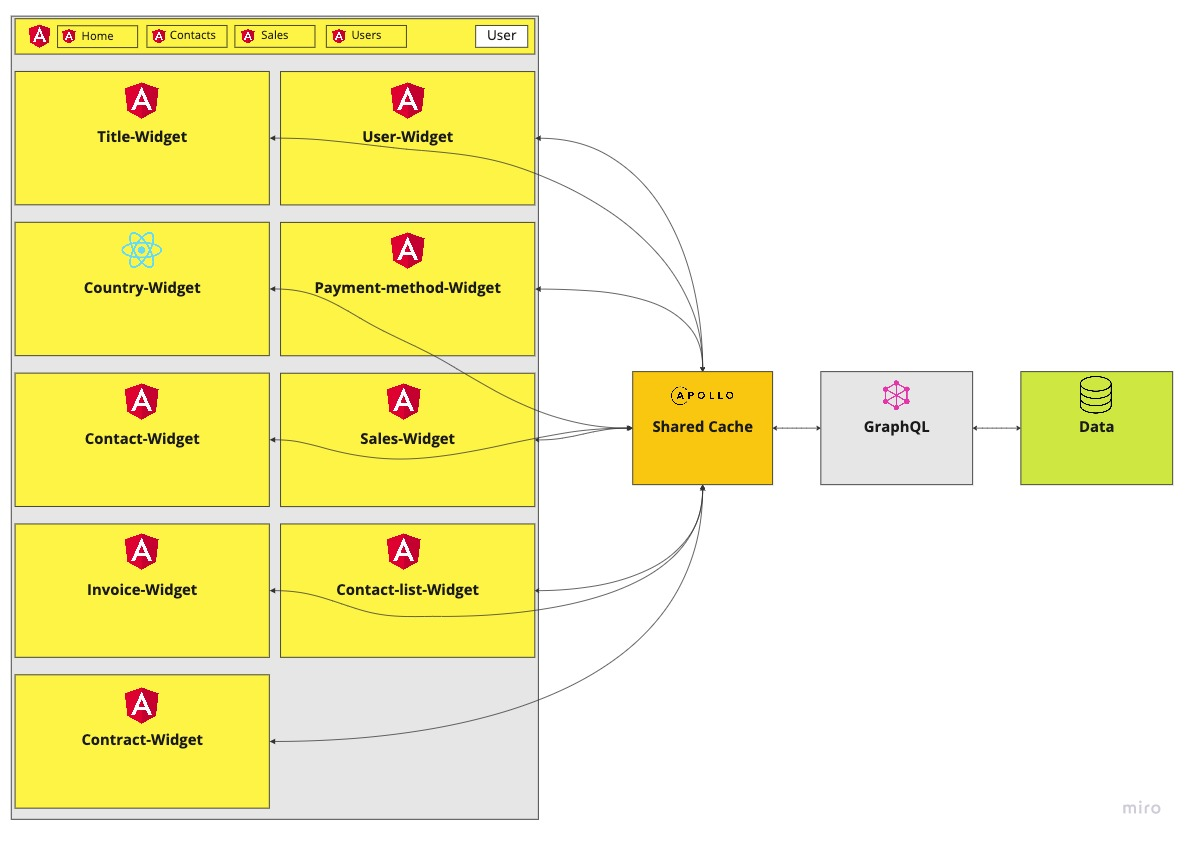
\includegraphics[width=0.8\linewidth]{images/ui-dashboard-architecture.jpg}
\caption{Architecture of the micro-frontend prototype.}\label{figure:methods:ui-dashboard-architecture}
\end{figure}
\fi

The functionality of the micro-frontends is encapsulated in modules that can be used by the shell application. Each icon of Angular and React represents such a module, as shown in figure \ref{figure:methods:ui-dashboard-architecture}. These modules can be used when the application is running in standalone mode, and the modules can be made accessible to the shell application via module federation.

\ifshowUnusedContent
% TODO(FM): Too detailed
% How a module can be exposed to be consumed by a remote application is shown in the listing \ref{code:methods:module-federation-config-expose}.

% \ifshowListings
% \begin{listing}[htbp]
% \begin{minted}{typescript}
% module.exports = {
%   name: 'contact',
%   exposes: {
%     './Module': 'apps/contact/src/app/remote-entry/entry.module.ts',
%   },
% };
% \end{minted}
% \caption{Module Federation config to expose an Angular module to be consumed.}\label{code:methods:module-federation-config-expose}
% \end{listing}
% \fi

% The host can configure its Module Federation to to be able to consume the entry.module.ts from the contact micro-frontend. The configuration can be seen in the listing \ref{code:methods:module-federation-config-consume}.

% \ifshowListings
% \begin{listing}[htbp]
% \begin{minted}{typescript}
% module.exports = {
%   name: 'host',
%   remotes: {
%     contact: 'contact@http://localhost:4202/remoteEntry.js'
%   },
% };
% \end{minted}
% \caption{Module Federation config that consumes an Angular module from a remote location.}\label{code:methods:module-federation-config-consume}
% \end{listing}
% \fi

% Inside the host application the remote module from the contact application can be easily referenced and routed to. The configuration of the route can be seen in listing \ref{code:methods:angular-route-to-remote-module}

% \ifshowListings
% \begin{listing}[htbp]
% \begin{minted}{typescript}
% const routes: Routes = [
%   {
%     path: 'contact',
%     loadChildren: () => 
%     loadRemoteModule(
%       'contact', 
%       './Module'
%     ).then((m) => m.UiContactRemoteEntryModule),
%   },
% }
% \end{minted}
% \caption{Route to the exposed remote-module from the contact application}\label{code:methods:angular-route-to-remote-module}
% \end{listing}
% \fi
\fi

\section{Communication from the shell- to the remote-application}\label{section:methods:communication-shell-remote}

To solve the problem of building a common caching layer, some form of communication between the shell and remote application had to be implemented. To ensure that the micro-frontends remain independent of each other, it should be avoided that they communicate directly with each other.

Angular provides a great tool for this use case, namely dependency injection. The shell application can provide services that can later be injected by the remote applications. This is very handy because the micro frontend can provide the same services as the shell application in standalone mode. Therefore, the remote module can be easily used within the remote and shell application.

\ifshowUnusedContent
% TODO(FM): Too detailed
% For example i implemented a layout-service that takes advantage of dependency injection. 

% \ifshowImages
% \begin{figure}[!htbp]
% \centering
% 
\includegraphics[width=1\linewidth]{images/prototype-screenshots/contact-header.png}
% \caption{Beispiel für die Beschriftung eines Buchrückens.}
% \end{figure}
% \fi

% \ifshowImages
% \begin{figure}[!htbp]
% \centering
% 
\includegraphics[width=1\linewidth]{images/prototype-screenshots/host-contact-header.png}
% \caption{Beispiel für die Beschriftung eines Buchrückens.}
% \end{figure}
% \fi
\fi

\section{Shared caching layer between the micro-frontends}

With the knowledge from the previous section \ref{section:methods:communication-shell-remote} a shared caching layer was implemented. Apollo GraphQL was chosen as GraphQL client for this prototype. It offers the most support for various frameworks and has a large community. The shell application can provide the instance of the GraphQL cache, which the micro-frontends can inject and use, when setting up their client, as seen in figure \ref{code:methods:graphql-client-cache-provider}. When running the micro-frontend in standalone mode, this provider has to be used inside the native application of the micro-frontend.

\ifshowUnusedContent
% TODO(FM): Too detailed
% For example the contact-application provides this object seen in listing \ref{code:methods:graphql-client-cache-provider} in its providers-array inside the core.module.ts. The host-application has the exactly same configuration inside its core.module.ts.
\fi

\ifshowListings
\begin{listing}[H]
\begin{minted}{typescript}
@NgModule({
  providers: [
    {
      provide: UI_GRAPHQL_CLIENT_CACHE,
      useValue: new InMemoryCache(),
    },
  ],
})
export class UiContactCoreModule {}
\end{minted}
\caption{Provide the instance of the cache to dependency injection.}\label{code:methods:graphql-client-cache-provider}
\end{listing}
\fi

\ifshowUnusedContent
% TODO(FM): Too detailed
% UI\_GRAPHQL\_CLIENT\_CACHE is an Angular Injection-token that can be used to provide injectable objects that can be used with dependency injection. (TODO: Injection token link)

% These provider must only be set inside the providers of the core.module.ts that the native application provides. Otherwise the remote-module would have their own instances of the GraphQL cache and the shared caching-layer would not work. 
\fi

Every micro-frontend can have their own instance of a GraphQL client. Only the GraphQL cache is shared between the different applications. Therefore, in theory, it is also possible that every micro-frontend consumes a different GraphQL API. 

\ifshowUnusedContent
% TODO(FM): Too detailed
% \ifshowListings
% \begin{listing}[htbp]
% \begin{minted}{typescript}
% @NgModule({
%   providers: [
%     {
%       provide: UI_GRAPHQL_CLIENT_OPTIONS_CONFIG,
%       useValue: {
%         shareCache: true,
%         persistCache: false,
%         useTypePolicies: true,
%         typePolicies: UI_CONTACT_APP_TYPE_POLICIES,
%       } as UiGraphQLClientOptionsConfig,
%     },
%   ],
% })
% export class UiContactRemoteCoreModule {}
% \end{minted}
% \caption{Extra configuration TODO}\label{code:methods:graphql-client-extra-configuration-options}
% \end{listing}
% \fi
\fi

To make it simple for the micro-frontends to use GraphQL, a function was written that creates the GraphQL client, seen in listing \ref{code:methods:graphql-client-creation}.

\ifshowListings
\begin{listing}[H]
\begin{minted}{typescript}
UiGraphQLClientOptionsModule.withConfig('contact-remote-app', { 
  provideGraphQLClientOptions: true,
}),
\end{minted}
\caption{Provide the instance of the cache as injectable.}\label{code:methods:graphql-client-creation}
\end{listing}
\fi

The first parameter of the function is a unique name for the GraphQL client instance. The unique name is mostly used for logging purposes. The second parameter is a configuration object whose options can be configured that no client is created.  

\ifshowUnusedContent
% For example the GraphQL client could be already provided inside the core-module of the shell-application and the remote-application injects that instance of the GraphQL client. These configuration options were largely added to test the shared caching layer with different options.
\fi

The final architecture follows the approach that each micro-frontend has a separate GraphQL client and a shared cache. This allows for the most flexibility as the GraphQL client can be configured individually by each micro frontend.


\ifshowUnusedContent
% My prototype creates 12 GraphQL clients, if every remote-application is loaded.

% \begin{enumerate}
%   \item host-native-app-graphql-client
%   \item contact-remote-app-graphql-client
%   \item sales-remote-app-graphql-client 
%   \item user-remote-app-graphql-client 
%   \item address-remote-widget-graphql-client
%   \item contact-list-remote-widget-graphql-client
%   \item contact-remote-widget-graphql-client 
%   \item contract-remote-widget-graphql-client
%   \item invoice-remote-widget-graphql-client 
%   \item person-remote-widget-graphql-client 
%   \item sales-remote-widget-graphql-client
%   \item user-remote-widget-graphql-client 
% \end{enumerate}
\fi

\section{Built a mechanism that reduces the size of queries}

Apart from sharing a cache instance, performance can be improved even further when using GraphQL in a shared architecture by removing fields from a query that are already in the cache.
However, the Apollo GraphQL client and no other GraphQL client with a caching layer provides this feature out of the box. Caching in Apollo works at the query level. So when a query is executed against the GraphQL backend, the results of the query are cached. If the same query is executed again, the cache is queried first to determine whether the query is already contained. If all queried fields of the new and old query are identical, the query results in a cache hit. However, if the new query queries fields that have not yet been queried by the old query and are therefore not yet in the cache, the query will result in a cache miss and fetched from the server. Consequently, identical queries that fetch different fields are always fetched from the server.

Consider the listing \ref{code:methods:query-all-users-reduction}. The left query fetches all users, and the right query fetches a user by id. Both queries fetch the same data, but two requests to the backend are made. The second query could completely be omitted, if the caching layer would be taken advantage of.

% For this case Apollo offers cache redirects, but the redirect works only if the list- and detail-view query the exact same fields. For example if the user micro-frontend query a list of users seen in listing \ref{code:methods:query-all-users-reduction} and when a user is selected, the detail-view might display the individual user like in listing \ref{code:methods:query-single-user}.

\ifshowListings
\begin{listing}[H]
\begin{minted}{typescript}
query {                                query User(id: ID!) {
  allUsers {                              User(id: id) {
    id                                      id
    username                                username
    email                                   email
    firstName                               firstname
    secondName                              secondName
  }                                       }    
}                                      }
\end{minted}
\caption{Query all users for the list-view.}\label{code:methods:query-all-users-reduction}
\end{listing}
\fi

\ifshowUnusedContent
% TODO(FM): too detailed
% In this case it is known that the user-data is already inside the cache, but fetched by a different query. The Apollo client doesn't know that and therefore tries to fetch the User from the server. But with Type-Policies we can tell the Apollo client where to look for the cached User. How to write such a redirect is shown in listing \ref{code:methods:user-cache-redirect}.

% \ifshowListings
% \begin{listing}[H]
% \begin{minted}{typescript}
% const client = new ApolloClient({
%   cache: new InMemoryCache({
%     typePolicies: {
%       Query: {
%         fields: {
%           User(_, { args, toReference }) {
%             return toReference({
%               __typename: 'User',
%               id: args.id,
%             });
%           }
%         }
%       }
%     }
%   })
% });
% \end{minted}
% \caption{Writing a cache-redirect for the User-type}\label{code:methods:user-cache-redirect}
% \end{listing}
% \fi

% That a detail-view and a list-view are identical is very rare in applications. Therefore this approach can't be used to reduce the size of network-requests effectively. And the approach is very verbose, because this redirect has to be written for every object type.
\fi

Many feature requests in the Apollo repository call for such a feature. While browsing GitHub, I found a project that provides drop-in replacements for Apollo's GraphQL query methods. And it provides the functionality to remove fields from a query that are already in the cache. However, the big problem was that the project was developed specifically for React and the dependencies were outdated. As a result, I couldn't install it and use it within the micro frontend written in React.

The next step was to rewrite the library in TypeScript and update the dependencies. While rewriting the library, some new features were added to still be able to exploit the cache-layer.

% But the library lacked the feature of cache-redirects. Therefore, the fields which were already queried by a list-view, couldn't be reduced when the detail-view was queries. I enhanced the implementation by adding a parameter, where a reference to an existing cache-object can be specified. If no reference is found in the cache, these reference to a cache-object is used to reduce the query.

In contrast to the original implementation, the new implementation is technology agnostic and can be used with every frontend framework that supports the Apollo client. For ease of use, I wrote adapters for React and Angular that have the same API as Apollo's original methods. The next section shows an example of the library in action.

\subsection{Example reduction}

This section contains an example of how query reduction works. The user navigates to the list view of all users, which executes the GraphQL query shown in listing \ref{code:methods:query-all-users}. After the query is fetched from the GraphQL backend, the fields in the query are cached

\ifshowListings
\begin{listing}[H]
\begin{minted}{typescript}
query allUsers {
  allUsers {
    id
    username
    email
    password
    firstName
    secondName
    gender
    Title {
      id
    }
    Salutation {
      id
    }
  }
}
\end{minted}
\caption{GraphQL query that queries all users.}\label{code:methods:query-all-users}
\end{listing}
\fi

The user then navigates to the detail view of a particular user. The left GraphQL query shown in the figure \ref{figure:code:comparison-user-reduced-user} is the original query that would normally be fetched from the backend. But with the help of reducing of the query with already existing data the right query is sent instead to the backend. Exactly the fields which were queried with the GraphQL query shown in listing \ref{code:methods:query-all-users} are removed. Therefore, 8 of the 16 fields were removed, reducing the size of the query by 50\%. In the next section, comparisons are made between the original queries and their reduced counterparts.

\ifshowImages
\begin{figure}[H]
\centering
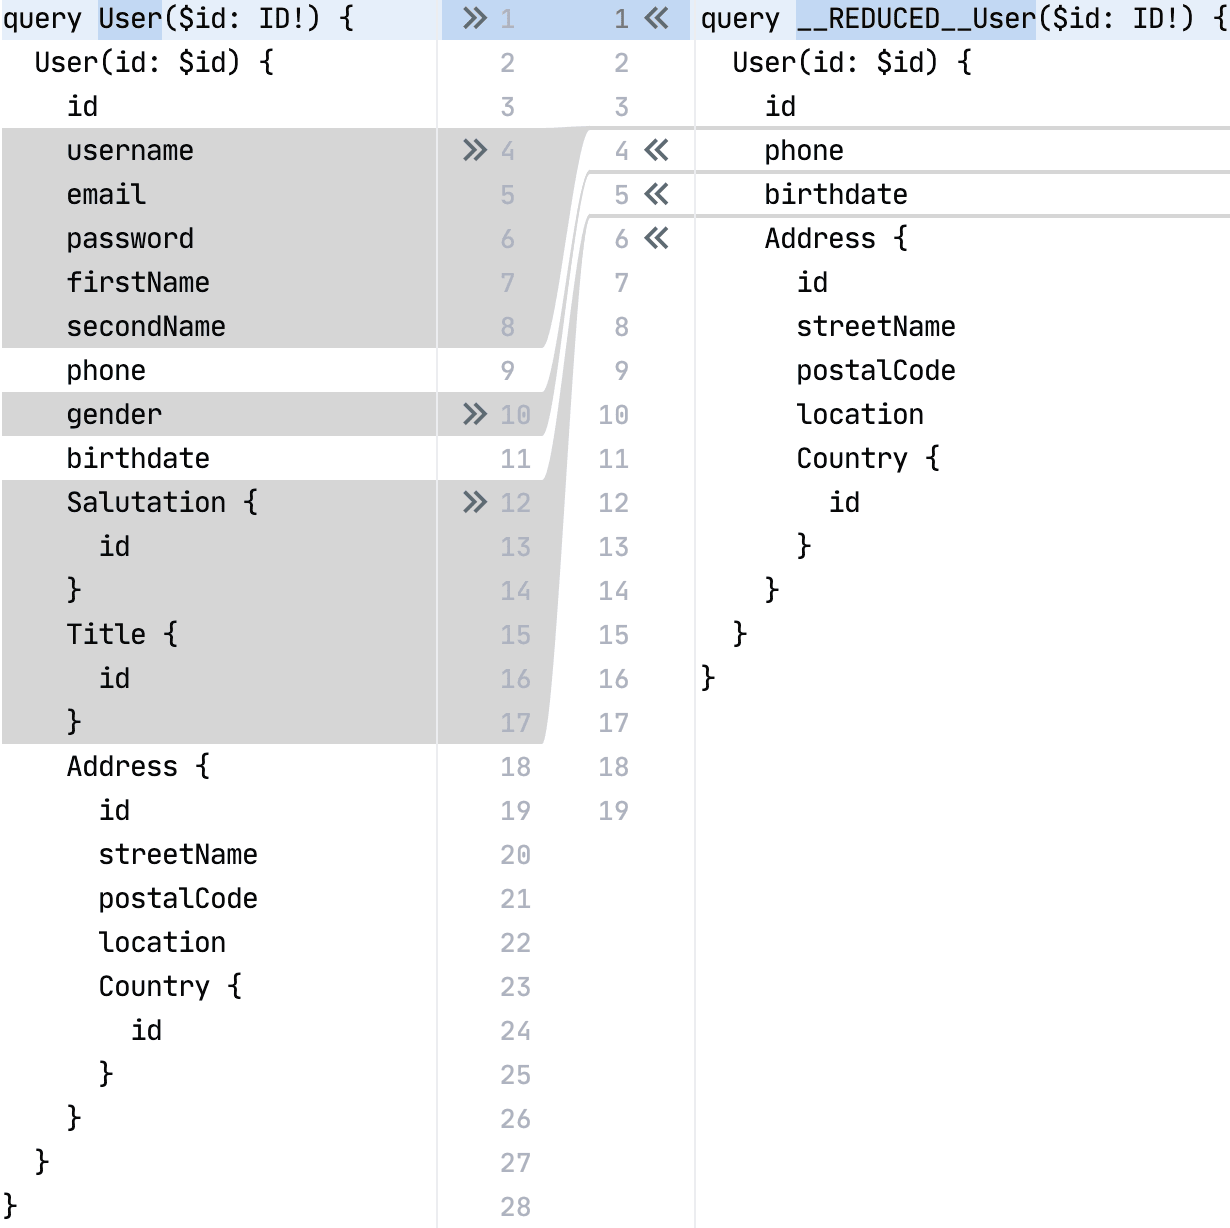
\includegraphics[width=0.6\linewidth]{images/reduction-graphql-examples/compare-user-reduced-user.png}
\caption{Comparison of the original user- and reduced user-query.}\label{figure:code:comparison-user-reduced-user}
\end{figure}
\fi

\subsection{Comparison between queries and reduced queries}

This section shows the difference in request- and response-size of different queries. The table \ref{table:code:comparison-user-reduction} shows the difference in size of the user-detail query, with the query reduction that was explained in the previous section. By removing 8 fields from the request, the size of the requests were reduced by 30\% or by 161 bytes. When querying 10 users a total of 1.61 KB can be saved. The response-size is reduced by 42\% on average. 2.55 KB in response-size is saved if 10 users are queried.

\ifshowTables
\begin{table}[H]
  \begin{tabular}{|l|l|l|l|l|}
  \hline
  Query & Request Diff (\%) & Request Diff (B) & Response Diff (\%) & Response Diff (B) \\
  \hline
  User & 30\% & 161 & 42\% & 257 \\
  \hline
  User & 30\% & 161 & 42\% & 257 \\
  \hline
  User & 30\% & 161 & 41\% & 257 \\
  \hline
  User & 30\% & 161 & 42\% & 244 \\
  \hline
  User & 30\% & 161 & 43\% & 251 \\
  \hline
  User & 30\% & 161 & 42\% & 271 \\
  \hline
  User & 30\% & 161 & 42\% & 249 \\
  \hline
  User & 30\% & 161 & 41\% & 263 \\
  \hline
  User & 30\% & 161 & 41\% & 248 \\
  \hline
  User & 30\% & 161 & 41\% & 252 \\
  \hline
  \hline
  \textbf{AVG} & \textbf{30\%} & - & \textbf{42\%} & -  \\
  \hline
  \textbf{SUM} & - & \textbf{1610 (1.61 KB)} & - & \textbf{2549 (2.55 KB)} \\
  \hline
  \multicolumn{5}{l}{16 fields, 8 Fields Removed, 8 remaining}
  \end{tabular}
  \caption{Comparison of the user-detail query in request- and response-sizes.}\label{table:code:comparison-user-reduction}
\end{table}
\fi

\ifshowUnusedContent
% TODO(FM): Too detailed
% The table \ref{table:code:comparison-contract-reduction} shows the difference for the contract-detail query. By running the list-query for all contracts 10 fields from the 17 can be removed from the query. Therefore only 7 from the 17 fields are remaining inside the query. The requests can be reduced by an average of 38\% or by 207 bytes. When using the application and querying 10 detail-views of the contract 2.07 KB can be saved. The size of the response from the GraphQL backend can be reduced by about 58\%. 3.96 KB in response-size is saved if 10 contracts are queried.

% \ifshowTables
% \begin{table}[ht]
%   \begin{tabular}{|l|l|l|l|l|}
%   \hline
%   Query  & Request Diff (\%)  & Request Diff (B) & Response Diff (\%) & Response Diff (B)  \\
%   \hline
%   Contract & 38\% & 207 & 58\% & 394 \\
%   \hline
%   Contract & 38\% & 207 & 58\% & 378 \\
%   \hline
%   Contract & 38\% & 207 & 59\% & 403 \\
%   \hline
%   Contract & 38\% & 207 & 60\% & 408 \\
%   \hline
%   Contract & 38\% & 207 & 60\% & 409 \\
%   \hline
%   Contract & 38\% & 207 & 57\% & 370 \\
%   \hline
%   Contract & 38\% & 207 & 58\% & 393 \\
%   \hline
%   Contract & 38\% & 207 & 58\% & 407 \\
%   \hline
%   Contract & 38\% & 207 & 59\% & 400 \\
%   \hline
%   Contract & 38\% & 207 & 58\% & 389 \\
%   \hline
%   \hline
%   \textbf{AVG} & \textbf{38\%} & - & \textbf{58\%} & - \\
%   \hline
%   \textbf{SUM} & - & \textbf{2070 (2.07 KB)} & - & \textbf{3951 (3.95 KB)} \\
%   \hline
%   \multicolumn{5}{l}{17 fields, 10 Fields Removed, 7 remaining}
%   \end{tabular}
%   \caption{Comparison of the contract-detail query in request- and response-sizes}\label{table:code:comparison-contract-reduction}
% \end{table}
% \fi

% \section{Persist the state of the cache}
% \section{Compared multiple GraphQL clients}
\fi

\chapter{Results}\label{chapter:results}

This chapter measures whether a micro-frontend with GraphQL and a shared caching layer can provide a performance improvement for the prototype implementation of the micro-frontend architecture. 

\section{Performance measurement}

Three different approaches were identified to measure the performance of the shared GraphQL caching layer.

\begin{enumerate}
    \item Separate Cache and no reduced queries
    \item Shared Cache and no reduced queries
    \item Shared Cache and reduced queries
\end{enumerate}

To measure the performance of these three approaches, two exemplary paths through the application were created. These examples were intended to show how many network requests were made to the GraphQL backend and how much network traffic was generated.

To make the measurement as close as possible to a real application, a large amount of data was added to the GraphQL backend. With this amount of data, it is easier to measure the difference in response size. The next section details the results of the first path through the application.

\subsection{Evaluation}

The following steps show the first path through the application. 

\begin{enumerate}
    \item Open Dashboard
    \item Open Contacts
    \item Open second Contacts page
    \item Open the first contact on the second page
    \item Open Invoices
    \item Open second Invoices page
    \item Open the first invoice on the second page
    \item Open Contracts
    \item Open second Contracts page
    \item Open the first Contract on the second page
    \item Open Users
    \item Open second Users page
    \item Open the first User on the second page
\end{enumerate}

For the path through the application \textbf{59} GraphQL queries would have to be executed against the backend, if no caching mechanism were in place. The next sections highlight the results in more detail.

\ifshowUnusedContent
% To make the testing process easier, I wrote a provider that allows me to easily change the settings to match one of the three approaches. As shown in listing \ref{listing:results:graphql-client-configuration} the UI\_GRAPHQL\_CLIENT\_OPTIONS\_CONFIG injection-token can be used to set if the cache should be should be shared (shareCache) or if a new instance of the cache should be provided. The settings of UI\_REDUCE\_QUERY\_OPTIONS (reduceQueries) can be used, whether the queries should be reduced with the data already inside the cache or not.

% \ifshowListings
% \begin{listing}[htbp]
% \begin{minted}{typescript}
% @NgModule({
%   provide: [
%     {
%       provide: UI_GRAPHQL_CLIENT_OPTIONS_CONFIG,  
%       useValue: {  
%         shareCache: false,  
%         persistCache: false,  
%         useTypePolicies: true,  
%         typePolicies: UI_DASHBOARD_APP_TYPE_POLICIES,  
%       } as UiGraphQLClientOptionsConfig,  
%     },  
%     {  
%       provide: UI_REDUCE_QUERY_OPTIONS,  
%       useValue: {  
%         reduceQueries: false,  
%       } as UiReduceQueryOptions,  
%     }
%    ],
% })
% export class UiContactRemoteCoreModule {}
% \end{minted}
% \caption{Providers to configure the behavior of the cache and query-reduction}\label{listing:results:graphql-client-configuration}
% \end{listing}
% \fi

% \begin{itemize}
%     \item allEmailTypes: 1
%     \item allSalutations: 5
%     \item allContactsSubset: 1
%     \item contactTitlesAggregated: 1
%     \item allTitles: 5
%     \item allContractsSubset: 1
%     \item allInvoicesSubset: 1
%     \item contactCountriesAggregated: 1
%     \item allCountries: 5
%     \item allArticleUnits: 3
%     \item allCurrencies: 3
%     \item allVats: 3
%     \item allSalesCountries: 5
%     \item allInvoiceTypes: 3
%     \item allUsersSubset: 1
%     \item \_allContactsMeta: 2
%     \item allContacts: 2
%     \item Contact: 1
%     \item \_allInvoicesMeta: 2
%     \item allInvoices: 2
%     \item Invoice: 1
%     \item \_allContractsMeta: 2
%     \item allContracts: 2
%     \item Contract: 1
%     \item \_allUsersMeta: 2
%     \item allUsers: 2
%     \item User: 1
% \end{itemize}
\fi

\subsubsection{Separate cache, no query reduction}

In this approach, each micro frontend has its own instance of the GraphQL client and cache. The queries are not reduced using the cache.

After completing the path through the applications, the Chrome Developer Tools provide the following metrics:

\begin{itemize}
    \item 47 GraphQL requests
    \item 10.7 MB transferred
\end{itemize}

\ifshowUnusedContent
%  To configure this behavior the following settings have to be provided to the UI\_GRAPHQL\_CLIENT\_OPTIONS\_CONFIG- and UI\_REDUCE\_QUERY\_OPTIONS injection-tokens inside the core-modules of the micro-frontend.

% \begin{itemize}
%     \item shareCache: false
%     \item reduceQueries: false
% \end{itemize}

% 47 requests have to be made to the GraphQL backend which can be seen in figure \ref{figure:results:no-shared-cache-no-reduction-chrome-dev-tools}. 6 of the 53 requests have to be removed, because these requests are done to load the other micro-frontends from their remote location. These requests are only needed for the functionality of the micro-service architecture.

% \ifshowImages
% \begin{figure}[!htbp]
% \centering
% 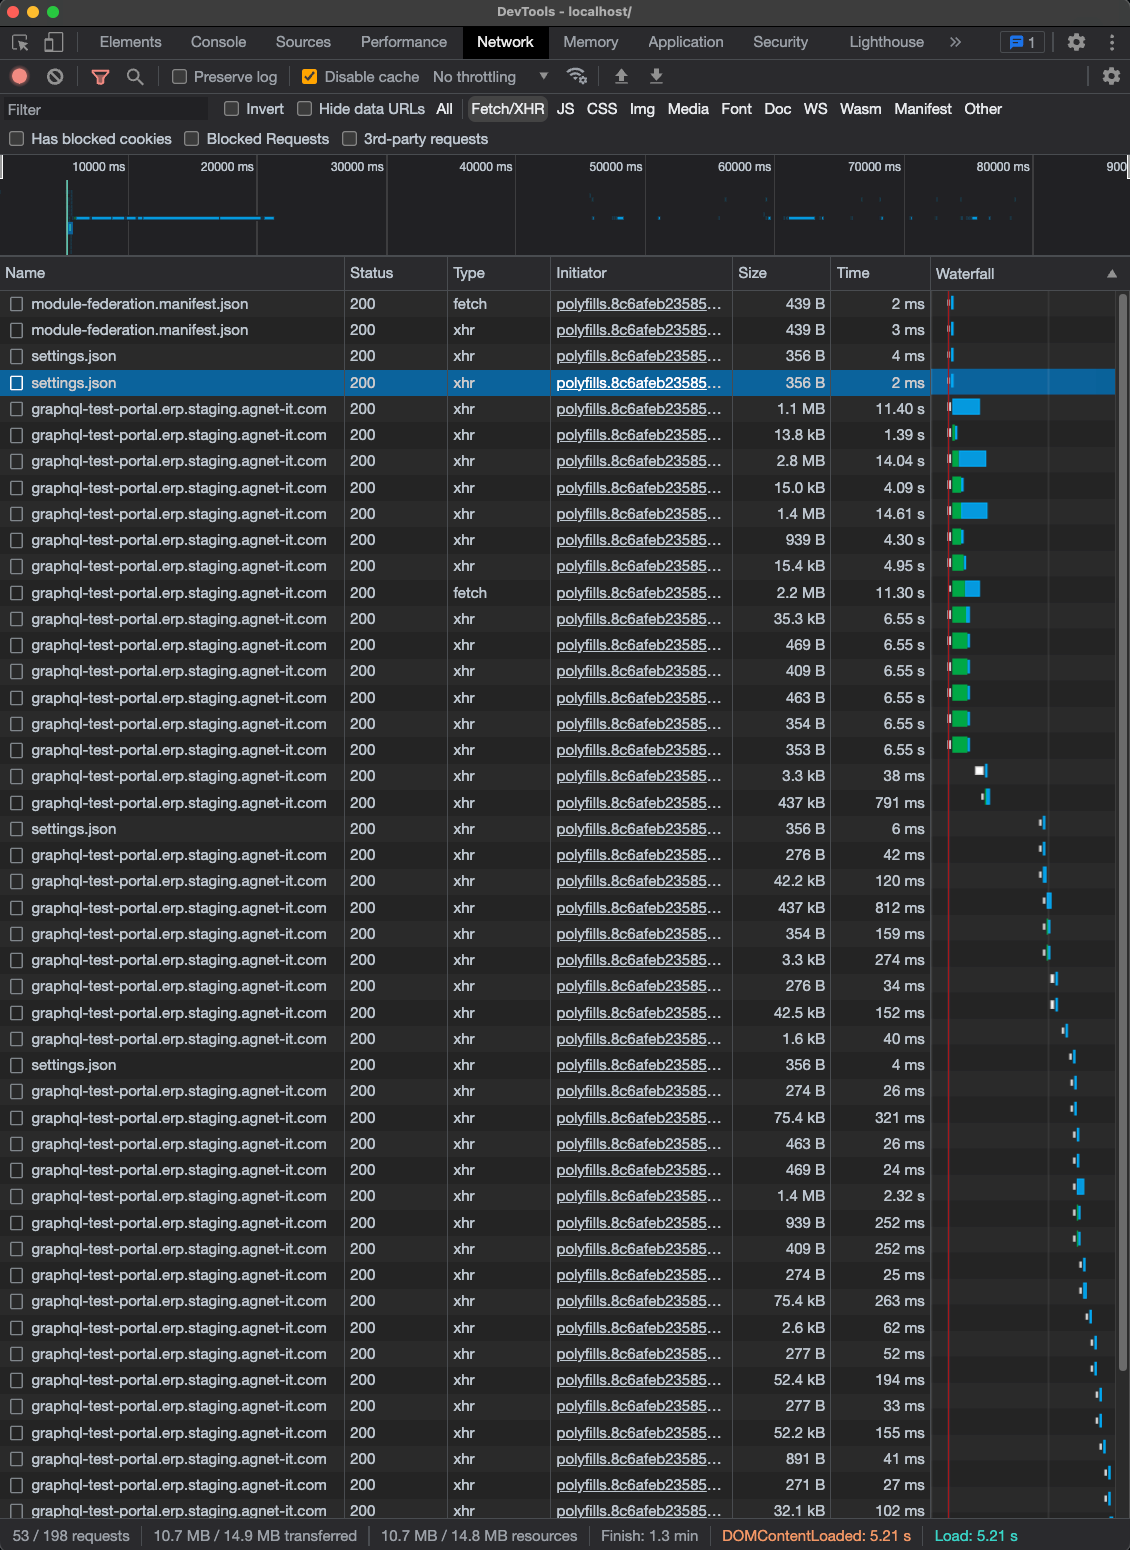
\includegraphics[width=0.6\linewidth]{images/1-attempt/no-shared-cache-no-reduction.png}
% \caption{All requests made during the measurement of the first approach}\label{figure:results:no-shared-cache-no-reduction-chrome-dev-tools}
% \end{figure}
% \fi
\fi

The total size of the queries was 17.46 KB and the size of the responses was 10.78 MB. The 47 queries retrieve a total of 61426 records from the GraphQL backend.

\subsubsection{Shared cache, no query reduction}

In this approach, the cache is shared by all micro-frontends and queries are not reduced by data already present in the cache.

After completing the path, the Chrome Developer Tools provide the following metrics:

\begin{itemize}
    \item 36 GraphQL requests
    \item 8.5 MB transferred
\end{itemize}

\ifshowUnusedContent
%  To configure this behavior the following settings have to be provided to the UI\_GRAPHQL\_CLIENT\_OPTIONS\_CONFIG- and UI\_REDUCE\_QUERY\_OPTIONS injection-tokens inside the core-modules of the micro-frontends.

% \begin{itemize}
%     \item shareCache: true
%     \item reduceQueries: false
% \end{itemize}

% 36 requests have to be made to the GraphQL backend which can be seen in figure \ref{figure:results:no-shared-cache-no-reduction-chrome-dev-tools}. 6 requests have to be subtracted (settings.json, module-federation.manifest.json) like previously.

% \ifshowImages
% \begin{figure}[!htbp]
% \centering
% 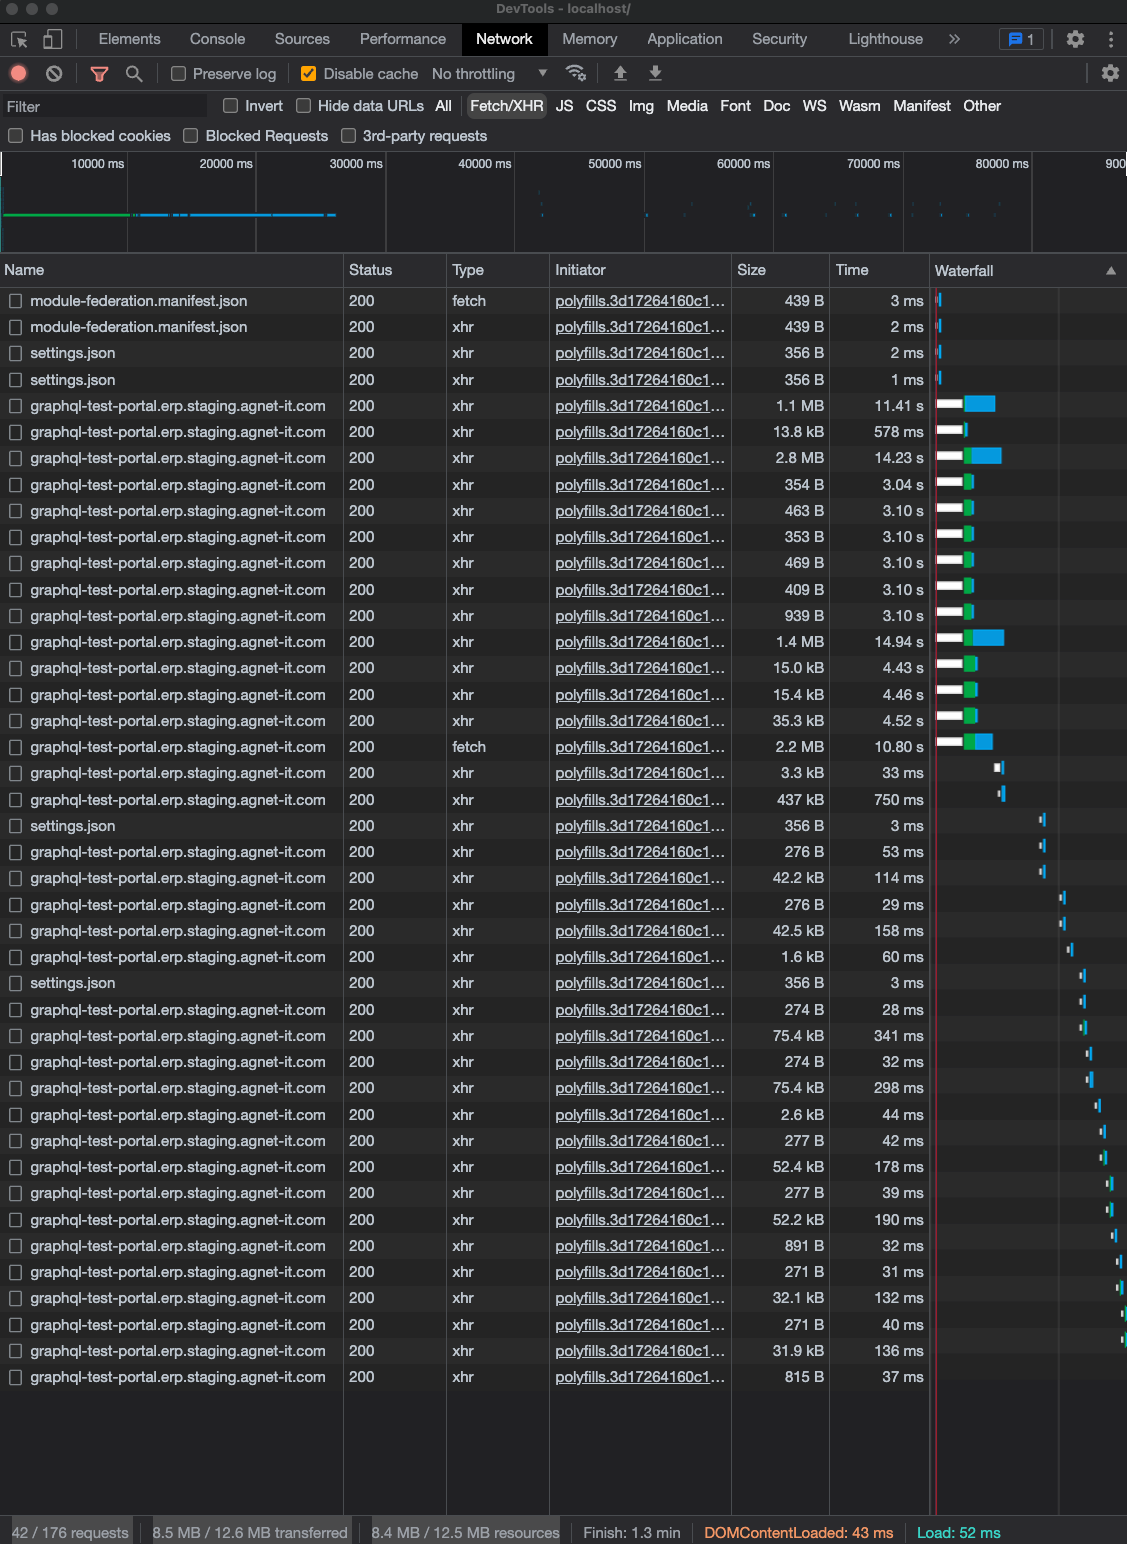
\includegraphics[width=0.6\linewidth]{images/1-attempt/shared-not-reduced-cache.png}
% \caption{All requests made during the measurement of the second approach}\label{figure:results:shared-cache-no-reduction-chrome-dev-tools}
% \end{figure}
% \fi
\fi

The total size of the queries was 15.176 KB and the size of the responses was 8.5 MB. The 36 queries retrieve a total of 51319 records from the GraphQL backend.

\subsubsection{Shared cache, query reduction}

With this approach, the cache is shared between all the micro-frontends and the queries are reduced with already existing data inside the cache.

After completing the path, the Chrome Developer Tools provide the following metrics:

\begin{itemize}
    \item 36 GraphQL requests
    \item 8.4 MB transferred
\end{itemize}

\ifshowUnusedContent
%  To configure this behavior the following settings have to be provided to the UI\_GRAPHQL\_CLIENT\_OPTIONS\_CONFIG- and UI\_REDUCE\_QUERY\_OPTIONS injection-tokens inside the core-modules of the micro-frontends.

% \begin{itemize}
%     \item shareCache: true
%     \item reduceQueries: false
% \end{itemize}

% 36 requests have to be made to the GraphQL backend which can be seen in figure \ref{figure:results:no-shared-cache-no-reduction-chrome-dev-tools}. 6 requests have to be subtracted (settings.json, module-federation.manifest.json).

% \ifshowImages
% \begin{figure}[!htbp]
% \centering
% 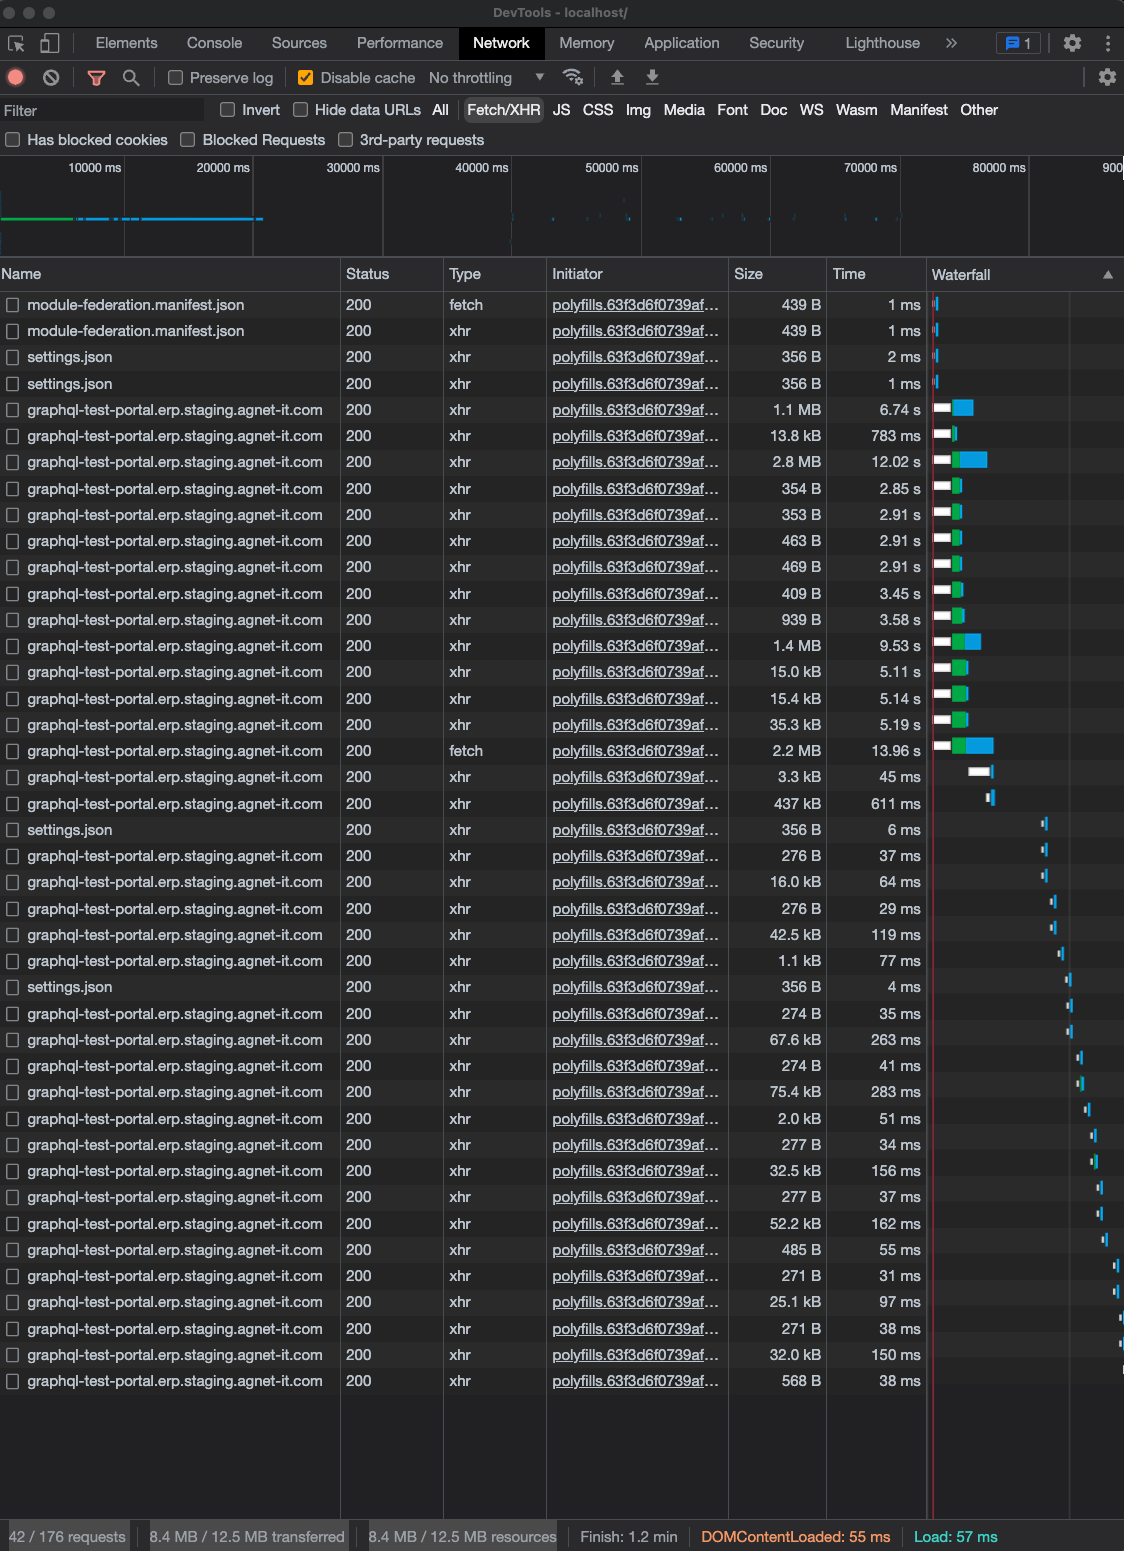
\includegraphics[width=0.6\linewidth]{images/1-attempt/shared-reduced-cache.png}
% \caption{All requests made during the measurement of the third approach}\label{figure:results:shared-cache-reduction-chrome-dev-tools}
% \end{figure}
% \fi
\fi

The total size of the queries was 13.533 KB and the size of the responses was 8.37 MB. The 36 queries retrieve a total of 51319 records from the GraphQL backend.

\subsubsection{Comparison between the three approaches}

This section compares compares the different approaches in terms of request- and response-size.

\paragraph{Comparing the first- and second-approach}

When comparing the first- with the second-approach there is a massive difference in the amount of network-requests made to the GraphQL backend and the size of the requests and responses, as seen in table \ref{table:results:size-comparison-first-path-no-cache-no-reduction-cache-no-reduction}. The shared cache approach requires 11 fewer network requests than the separate cache approach. Since the queries are not reduced in this comparison, the additional network queries account for the overall difference in request- and response-size. The 11 additional requests from the first approach send an additional 2.29 KB to the backend and return about an additional 2.34 MB from the backend. Therefore, 22\% of the total response-size can be saved by using only one shared cache. Another interesting observation is that the shared cache approach retrieves 10107 fewer records than the naive approach, which is 16\% of the total records returned.

\ifshowTables
\begin{table}[H]
    \begin{tabular}{|l|l|l|l|l|}
    \hline
      & Request Size (B) & Response Size (B) & Requests & Records \\
    \hline
     No Reduction, Separate Cache & 17462 & 10780656 & 47 & 61426 \\
     \hline
     No Reduction, Shared Cache & 15176 & 8437211 & 36 & 51319 \\
     \hline
     \hline
     \textbf{Diff} & \textbf{2286} & \textbf{2343445} & \textbf{11} & \textbf{10107} \\
     \hline
     \textbf{Reduction \%} & \textbf{13\%} & \textbf{22\%} & \textbf{23\%} & \textbf{16\%} \\
     \hline
    \end{tabular}
    \caption{Comparing the requests and responses of the first- and second-approach.}
    \label{table:results:size-comparison-first-path-no-cache-no-reduction-cache-no-reduction}
\end{table}
\fi

\ifshowUnusedContent
% TODO(FM): Too detailed
% Following requests have been omitted, when using a shared cache between the micro-frontends:

% \begin{itemize}
%     \item allCountries(User-MF, Contact-MF): 2
%     \item allSalutations(User-MF, Contact-MF): 2
%     \item allTitles(User-MF, Contact-MF): 2
%     \item allArticleUnits(Sales-MF): 1
%     \item allCurrencies(Sales-MF): 1
%     \item allVats(Sales-MF): 1
%     \item allSalesCountries(Sales-MF): 1
%     \item allInvoiceTypes(Sales-MF): 1
% \end{itemize}

% The data of the requests is usually used for filling select-controls inside detail-views and has to be fetched in every micro-frontends, when not using a shared-cache. The first three queries are used inside micro-frontends on the dashboard, the contact micro-frontend and the user micro-frontend. The last five queries are used inside micro-frontends on the dashboard and the sales micro-frontend.
\fi

\paragraph{Comparing the first- and third-approach}

Like in the previous comparison, there is also a massive difference in the amount of network-requests made to the GraphQL backend and the size of the requests and responses, as seen in table \ref{table:results:size-comparison-first-path-no-cache-no-reduction-cache-reduction}. Just like before, there is a difference in the 11 GraphQL queries that are sent to the backend. However, due to the reduction in queries, the difference in the size of the queries and responses is greater than before. All queries of the first approach send 3.92 KB more and return about 2.41 MB more from the backend compared to the third approach. A shared cache and query reduction can save about 22\% response size. As before, 16\% fewer records need to be fetched from the backend.

\ifshowTables
\begin{table}[H]
    \begin{tabular}{|l|l|l|l|l|}
    \hline
       & Request Size (B) & Response Size (B) & Requests & Records  \\
    \hline
     No Reduction, Separate Cache & 17462 & 10780656 & 47 & 61426 \\
     \hline
     Reduction, Shared Cache & 13533 & 8374763 & 36 & 51319 \\
     \hline
     \hline
     \textbf{Diff} & \textbf{3929} & \textbf{2405893} & \textbf{11} & \textbf{10107} \\
     \hline
    \textbf{Reduction \%} & \textbf{23\%} & \textbf{22\%} & \textbf{23\%} & \textbf{16\%} \\
     \hline
    \end{tabular}
    \caption{Comparing the requests and responses of the first- and third-approach.}
    \label{table:results:size-comparison-first-path-no-cache-no-reduction-cache-reduction}
\end{table}
\fi

\paragraph{Comparing the second- and third-approach}

Between the first- and the second-approach, there is almost no difference in request- and response-size compared to the other comparisons, as seen in table \ref{table:results:size-comparison-first-path-no-cache-no-reduction-cache-reduction}. As seen earlier, both approaches have the same number of queries since the cache is shared by all micro-frontends. Thus, the only difference in request and response size between the two approaches comes from the use of query reduction. By using the third approach, the size of the total requests is reduced by 1.64 KB (11\%). The difference between the response sizes (62.45 KB) is almost zero compared to the amount of data returned.

\ifshowTables
\begin{table}[H]
    \begin{tabular}{|l|l|l|l|l|}
    \hline
      & Request Size (B) & Response Size (B) & Requests & Records \\
    \hline
     No Reduction, Shared Cache & 15176 &  8437211 & 36 & 51319 \\
     \hline
     Reduction, Shared Cache &  13533 &  8374763 & 36 & 51319 \\
     \hline
     \hline
     \textbf{Diff} & \textbf{1643} & \textbf{62448} & \textbf{0} & \textbf{0} \\
     \hline
     \textbf{Reduction \%} & \textbf{11\%} & \textbf{0\%} & \textbf{-} & \textbf{-} \\
     \hline
    \end{tabular}
    \caption{Comparing the requests and responses of the second- and third-approach.}
    \label{table:results:size-comparison-first-path-cache-no-reduction-cache-reduction}
\end{table}
\fi

\ifshowUnusedContent
% \subsection{2. Attempt}

% The following enumeration shows the second path through the application. This attempt was made, with an authenticated user.

% \begin{enumerate}
%     \item Open Users
%     \item Open second Users page
%     \item Open the first User on the second page
%     \item Open the second User on the second page
%     \item Open Invoices
%     \item Open second Invoices page
%     \item Open the first invoice on the second page
%     \item Open the second invoice on the second page
%     \item Open Contracts
%     \item Open second Contracts page
%     \item Open the first Contract on the second page
%     \item Open the second Contract on the second page
%     \item Open Contacts
%     \item Open second Contacts page
%     \item Open the first Contact on the second page
%     \item Open the second Contact on the second page
%     \item Open Dashboard
% \end{enumerate}

% For this path through the application \textbf{59} queries in total have to be executed against the
% GraphQL backend, when no caching mechanism are implemented.

% \begin{itemize}
%     \item userByToken: 9
%     \item \_allUsersMeta: 2
%     \item allUsers: 2
%     \item allCountries: 5
%     \item allSalutations: 5
%     \item allTitles: 5
%     \item User: 2
%     \item \_allInvoicesMeta: 2
%     \item allInvoices: 2
%     \item allArticleUnits: 3
%     \item allCurrencies: 3
%     \item allVats: 3
%     \item allSalesCountries: 5
%     \item allInvoiceTypes: 3
%     \item Invoice: 2
%     \item \_allContractsMeta: 2
%     \item allContracts: 2
%     \item Contract: 2
%     \item \_allContactsMeta: 2
%     \item allContacts: 2
%     \item Contact: 2
%     \item allEmailTypes: 1
%     \item allContactsSubset: 1
%     \item contactTitlesAggregated: 1
%     \item allContractsSubset: 1
%     \item allInvoicesSubset: 1
%     \item contactCountriesAggregated: 1
%     \item allUsersSubset: 1
% \end{itemize}

% \begin{table}[]
%     \begin{tabular}{|l|l|l|l|}
%     \hline
%                                     & Request Size & Response Size & Request Amount  \\
%     \hline
%      No Reduction, Shared Cache     &  16884 B        &  8364416 B   & 37 \\
%      \hline
%      Reduction, Shared Cache        &  14718 B        &  8361306 B   & 37 \\
%      \hline
%     \textbf{Diff}                   & \textbf{2166 B (0.0016 MB)} & \textbf{3110 B (0.062  MB)} & \textbf{11} \\
%      \hline
%     \end{tabular}
%     \caption{Vergleich der State of the art Serious games.}
%     \label{tab:serious-game-comparison}
% \end{table}

% \begin{table}[]
%     \begin{tabular}{|l|l|l|l|}
%     \hline
%                                     & Request Size & Response Size & Request Amount  \\
%     \hline
%      No Reduction, No Shared Cache     &  22955 B        &  10713304 B   & 62 \\
%      \hline
%      Reduction, Shared Cache        &  14718 B        &  8361306 B   & 37 \\
%      \hline
%     \textbf{Diff}                   & \textbf{8237 B (0.0016 MB)} & \textbf{2351998 B (0.062  MB)} & \textbf{25} \\
%      \hline
%     \end{tabular}
%     \caption{Vergleich der State of the art Serious games.}
%     \label{tab:serious-game-comparison}
% \end{table}

% \begin{table}[]
%     \begin{tabular}{|l|l|l|l|}
%     \hline
%                                     & Request Size & Response Size & Request Amount  \\
%     \hline
%      No Reduction, No Shared Cache     &  22955 B        &  10713304 B   & 62 \\
%      \hline
%      No Reduction, Shared Cache        &  16884 B        &  8364416 B   & 37 \\
%      \hline
%     \textbf{Diff}                   & \textbf{6071 B (0.0016 MB)} & \textbf{2348888 B (0.062  MB)} & \textbf{25} \\
%      \hline
%     \end{tabular}
%     \caption{Vergleich der State of the art Serious games.}
%     \label{tab:serious-game-comparison}
% \end{table}
\fi

% \section{Stale data}


\chapter{Discussion}\label{chapter:discussion}

This project report investigated whether GraphQL can bring performance improvement in micro-frontend architectures. The results of the evaluation of the prototype implementation of the micro-frontend architecture are discussed in this chapter. The results from Chapter \ref{chapter:results} are used to make a statement about the hypothesis from Chapter \ref{chapter:introduction}.

\section{Request Size}

Figure \ref{figure:discussion:request-size} displays the results already shown in the previous chapter as a bar chart. In terms of request-size the three approaches are not very far apart from each other. The reduction of queries only makes 1.64 KB difference, in contrast to only sharing the cache.

\ifshowImages
\begin{figure}[H]
\centering
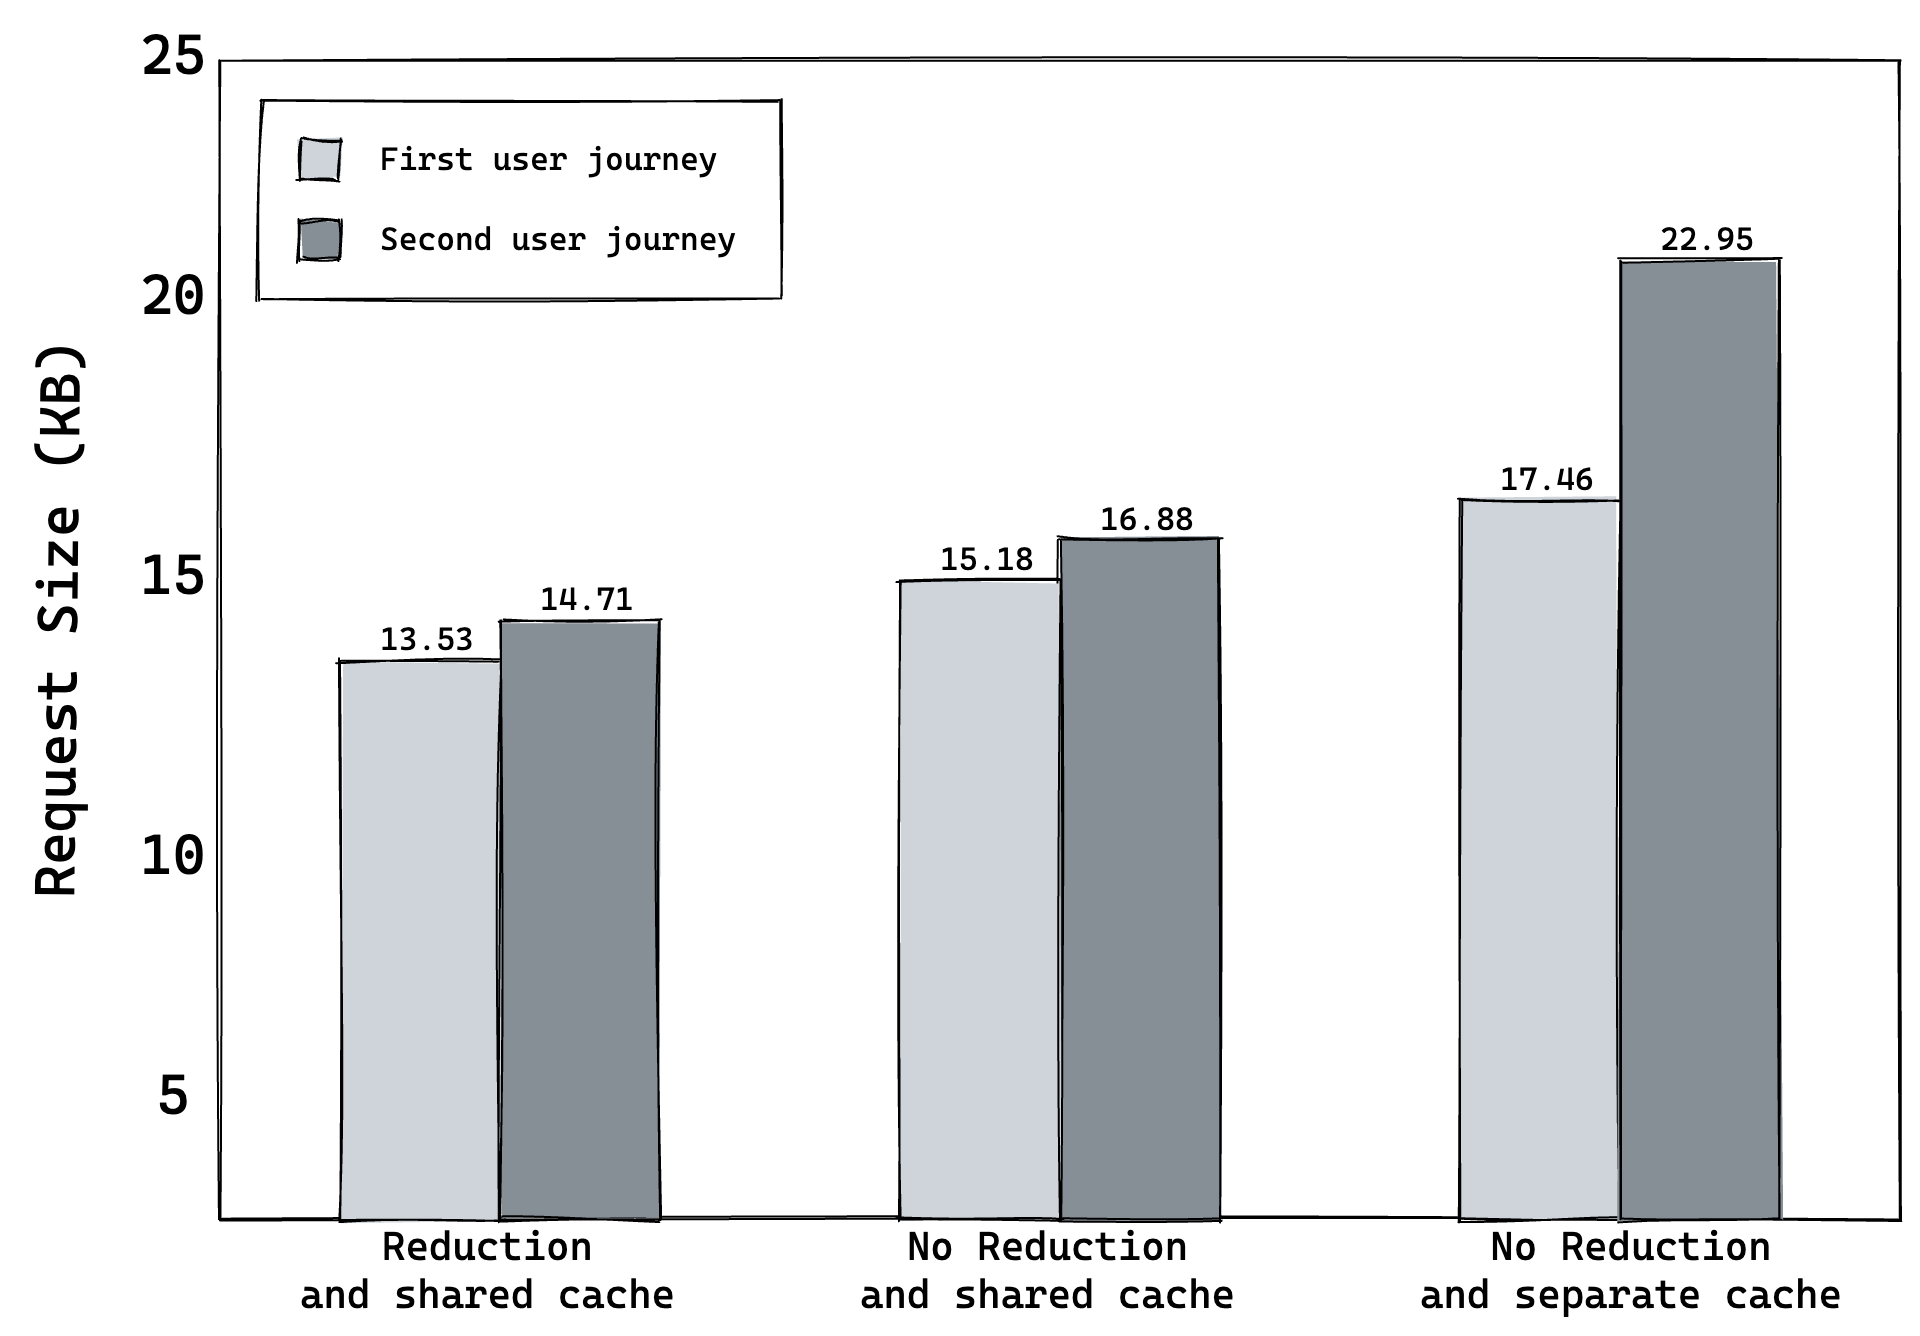
\includegraphics[width=0.8\linewidth]{images/discussion/request-size.png}
\caption{Request size comparison of the three approaches.}\label{figure:discussion:request-size}
\end{figure}
\fi

\section{Response Size}

Figure \ref{figure:discussion:response-size} displays the results already shown in the previous chapter as a bar chart. In contrast to the request-size, the response sizes are very far apart. When comparing the naive approach with the two improved approaches, there is a difference of about 2.40 MB. However, when comparing the two improved approaches, the difference is not very large. For the records that the application fetches, the reduction does not make such a big difference, in terms of responses.

\ifshowImages
\begin{figure}[H]
\centering
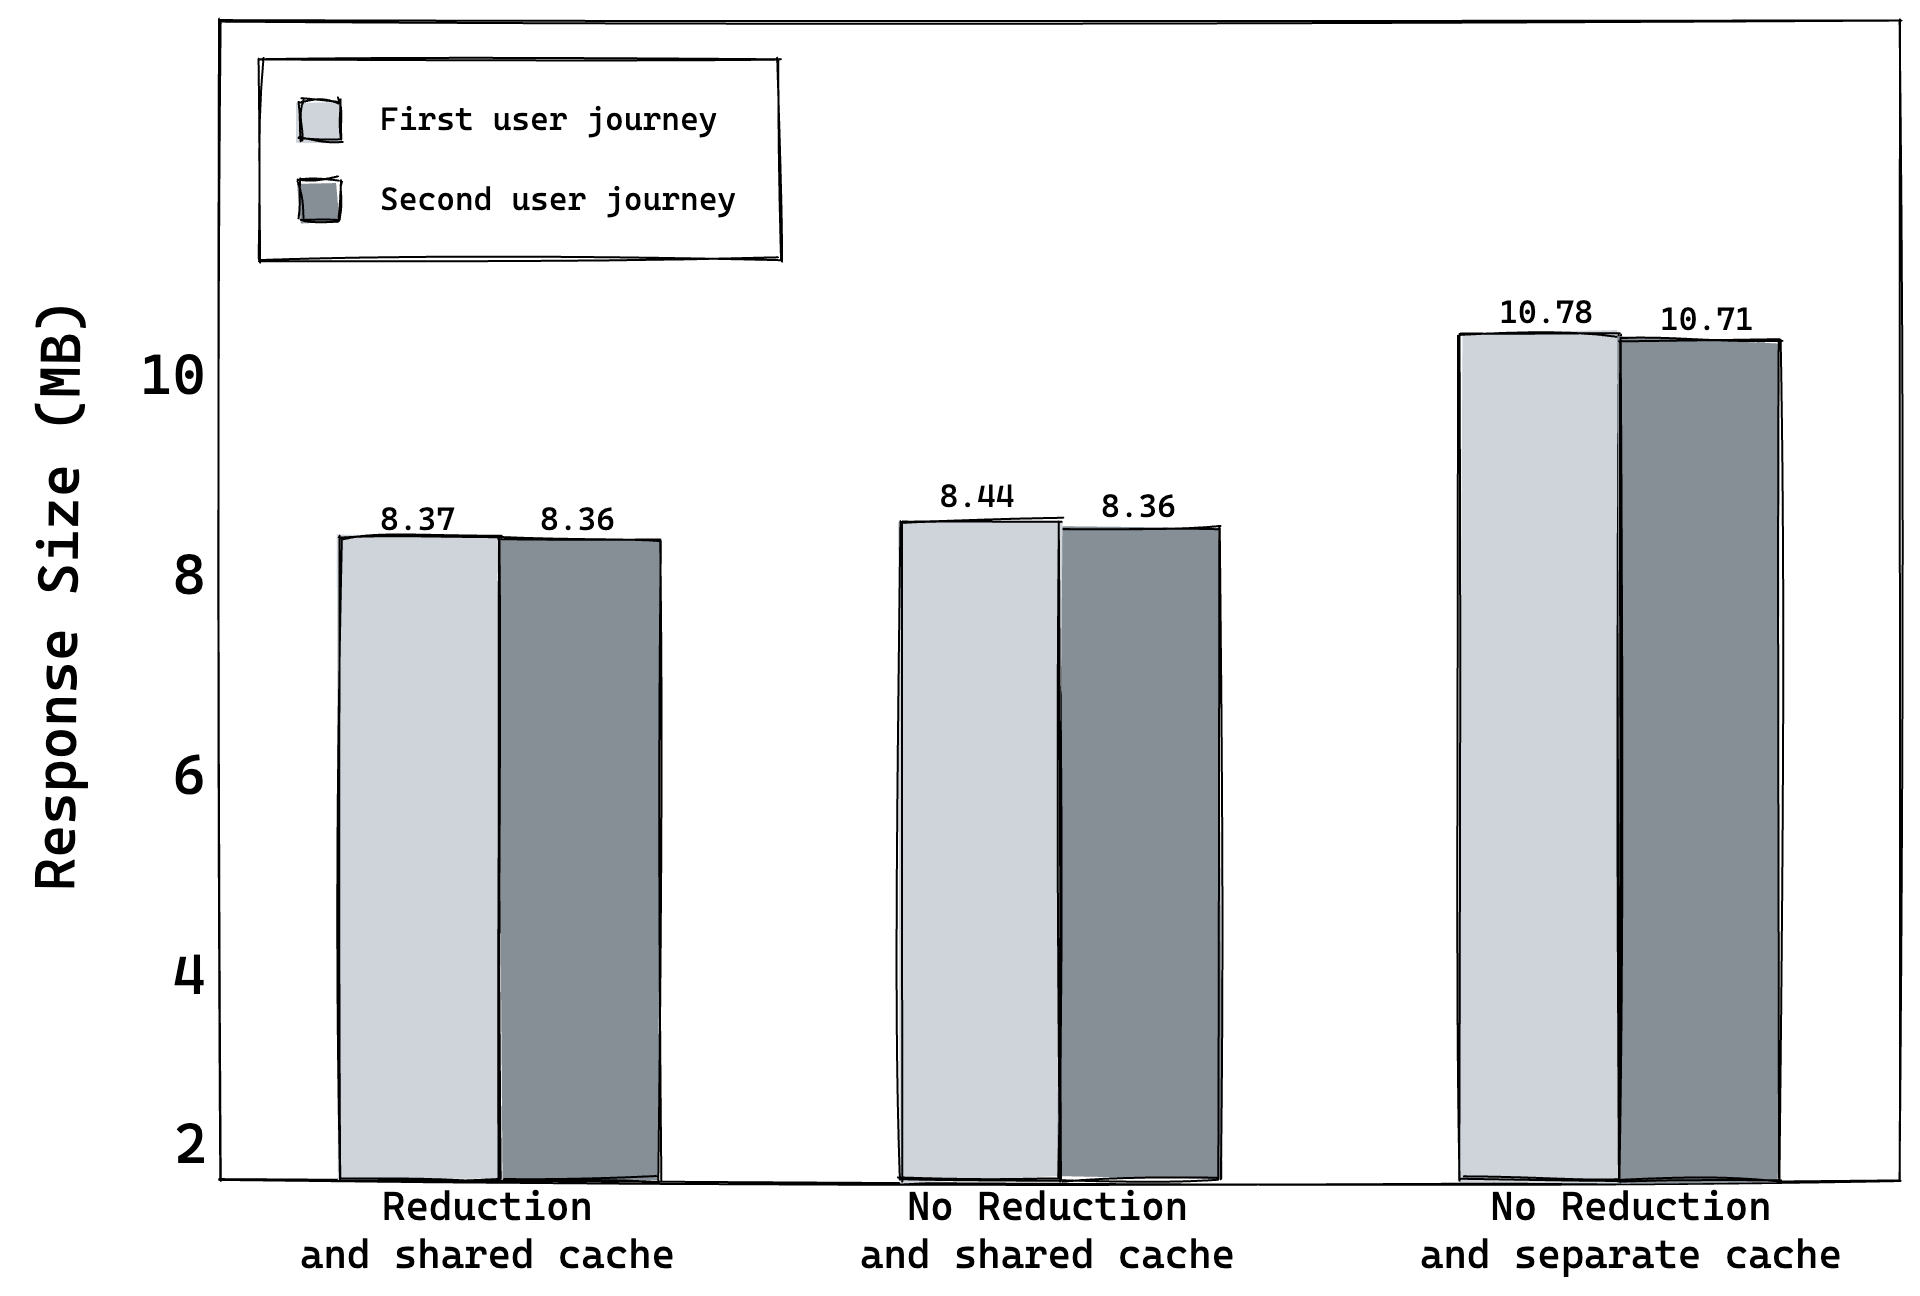
\includegraphics[width=0.8\linewidth]{images/discussion/response-size.png}
\caption{Response size comparison of the three approaches.}\label{figure:discussion:response-size}
\end{figure}
\fi

\chapter{Conclusion}\label{chapter:conclusion}

To validate the first hypothesis, which states that using GraphQL with a common caching layer can prevent over-fetching and over-requesting, a micro-frontend architecture with 12 different applications was designed and implemented. In the future, it is planned to integrate the prototype with AGnet's micro-frontend architecture. Therefore, the GraphQL queries used will be used later in the real application and the results of the evaluations are very expressive.\\

First, the shared caching layer was implemented, and to further improve performance, a mechanism was written to reduce queries with content already in the cache.\\

Based on the groundwork three different approaches were identified, how the prototype could be evaluated. Just sharing the cache between the micro-frontends resulted in a total save 22\% of response-size in comparison to a separated cache.\\

But the reduction in queries doesn't make that much difference with the queries in this prototype. The difference in request-size is only a few kilobytes, and the difference in response-size is not large enough to make a real difference.\\

To validate the second hypothesis, which states that the prototype should provide enough freedom in the choice of technology, a micro frontend was written using React and embedded in the shell application. The application was able to integrate with the existing architecture and use both the shared caching layer and the query reduction mechanism. The architecture is thus open to the free choice of technology.\\

%
% Hier beginnen die Verzeichnisse.
%
\clearpage
\printbibliography
\clearpage

% Das Abbildungsverzeichnis
\listoffigures
\clearpage

% Das Tabellenverzeichnis
\listoftables
\clearpage

% Das Quellcodeverzeichnis
\listoflistings
\clearpage

\phantomsection
\addcontentsline{toc}{chapter}{\listacroname}
\chapter*{\listacroname}
\begin{acronym}[XXXXX]
    % \acro{WWW}[WWW]{wor ld wide web}
\end{acronym}

%
% Hier beginnt der Anhang.
%
\clearpage
\appendix
\chapter{Anhang A}
\clearpage
\chapter{Anhang B}
\end{document}
